\documentclass[a4paper]{article}
\usepackage{vntex}
\usepackage{a4wide,amssymb,epsfig,latexsym,multicol,array,hhline,fancyhdr}
\usepackage{amsmath}
\usepackage{lastpage}
\usepackage[lined,boxed,commentsnumbered]{algorithm2e}
\usepackage{enumerate}
\usepackage{color}
\usepackage{graphicx}							% Standard graphics package
\usepackage{array}
\usepackage{tabularx, caption}
\usepackage{multirow}
\usepackage{multicol}
\usepackage{listings}
\usepackage{color}
\usepackage{rotating}
\usepackage{graphics}
\usepackage{geometry}
\usepackage{setspace}
\usepackage{epsfig}
\usepackage{tikz}
\usetikzlibrary{arrows,snakes,backgrounds}
\usepackage{hyperref}
\hypersetup{urlcolor=blue,linkcolor=black,citecolor=black,colorlinks=true} 
%\usepackage{pstcol} 								% PSTricks with the standard color package
\usepackage{gensymb}
\usepackage{tabularx}
\usepackage{float}

%\usepackage{fancyhdr}
\setlength{\headheight}{40pt}
\pagestyle{fancy}
\fancyhead{} % clear all header fields
\fancyhead[L]{
 \begin{tabular}{rl}
    \begin{picture}(25,15)(0,0)
    \put(0,-8){
\includegraphics[width=8mm, height=8mm]{hcmut.png}}
    %\put(0,-8){\epsfig{width=10mm,figure=hcmut.eps}}
   \end{picture}&
	%
\includegraphics[width=8mm, height=8mm]{hcmut.png} & %
	\begin{tabular}{l}
		\textbf{\bf \ttfamily Trường Đại Học Bách Khoa Tp.Hồ Chí Minh}\\
		\textbf{\bf \ttfamily Khoa Khoa Học và Kỹ Thuật Máy Tính}
	\end{tabular} 	
 \end{tabular}
}
\fancyhead[R]{
	\begin{tabular}{l}
		\tiny \bf \\
		\tiny \bf 
	\end{tabular}  }
\fancyfoot{} % clear all footer fields
\fancyfoot[L]{\scriptsize \ttfamily Bài tập lớn môn Mật mã và an ninh mạng}
\fancyfoot[R]{\scriptsize \ttfamily Trang {\thepage}/\pageref{LastPage}}
\renewcommand{\headrulewidth}{0.3pt}
\renewcommand{\footrulewidth}{0.3pt}


%%%
\setcounter{secnumdepth}{4}
\setcounter{tocdepth}{3}
\makeatletter
\newcounter {subsubsubsection}[subsubsection]
\renewcommand\thesubsubsubsection{\thesubsubsection .\@alph\c@subsubsubsection}
\newcommand\subsubsubsection{\@startsection{subsubsubsection}{4}{\z@}%
                                     {-3.25ex\@plus -1ex \@minus -.2ex}%
                                     {1.5ex \@plus .2ex}%
                                     {\normalfont\normalsize\bfseries}}
\newcommand*\l@subsubsubsection{\@dottedtocline{3}{10.0em}{4.1em}}
\newcommand*{\subsubsubsectionmark}[1]{}
\makeatother
%%%%
\definecolor{dkgreen}{rgb}{0,0.6,0}
\definecolor{gray}{rgb}{0.5,0.5,0.5}
\definecolor{mauve}{rgb}{0.58,0,0.82}
 
\lstset{frame=tb,
  language=Python,
  aboveskip=3mm,
  belowskip=3mm,
  showstringspaces=false,
  columns=flexible,
  basicstyle={\small\ttfamily},
  numbers=none,
  numberstyle=\tiny\color{gray},
  keywordstyle=\color{blue},
  commentstyle=\color{dkgreen},
  stringstyle=\color{mauve},
  breaklines=true,
  breakatwhitespace=true,
  tabsize=3
}
%%%%


\begin{document}

\begin{titlepage}
\begin{center}
ĐẠI HỌC QUỐC GIA THÀNH PHỐ HỒ CHÍ MINH \\
TRƯỜNG ĐẠI HỌC BÁCH KHOA \\
KHOA KHOA HỌC - KỸ THUẬT MÁY TÍNH 
\end{center}

\vspace{1cm}


\includegraphics[width=5cm]{hcmut.png}
\hfill

\includegraphics[width=5cm]{cse.png}

\vspace{1cm}


\begin{center}
\begin{tabular}{c}
\multicolumn{1}{l}{\textbf{{\Large MẬT MÃ VÀ AN NINH MẠNG}}}\\
~~\\
\hline
\\
\multicolumn{1}{l}{\textbf{{\Large Bài tập lớn 1}}}\\
\\
\textbf{{\Huge ỨNG DỤNG MÃ HÓA ĐƠN GIẢN}}\\
\\
\hline
\end{tabular}
\end{center}

\vspace{3cm}

\begin{center}
\begin{table}[h]
\begin{tabular}{rrll}
\hspace{5 cm} & GVHD: & Nguyễn Hữu Hiếu&\\
& SV: & Dương Tấn Sang &1512777\\
&&Lê Bá Anh Tuấn &1414384\\
&&Ngô Thiên Tín&...
\end{tabular}
\end{table}
\end{center}

\begin{center}
{\footnotesize TP. HỒ CHÍ MINH, THÁNG 4/2018}
\end{center}
\end{titlepage}


%\thispagestyle{empty}

\newpage
\tableofcontents
\newpage
\section{Các nội dung được trình bày trong báo cáo.}
\begin{itemize}
	\item
	Tìm hiểu các giải thuật mã hóa: Đối xứng(DES,AES), Bất đối xứng(RSA).
	\item
	Lý do chọn các giải thuật mã hóa và cơ sở lý thuyết.
	\item
	Tập tin mà chương trình  hỗ trợ mã hóa/ giải mã.
	\item
	Ngôn ngữ được sử dụng để hoàn thành.
	\item
	Hướng dẫn sử dụng phần mềm.
	\item
	Nhiệm vụ của các thành viên trong nhóm.
\end{itemize}
\section{Giới thiệu tổng quan về công việc đã làm.}
\begin{itemize}
	\item
	Công việc thực hiện dựa trên các giải thuật đã học, bằng cách sử dụng ngôn ngữ python để hoàn thành giao diện cho người dùng cùng với việc nhúng các mã vào giao diện.
	\item
	 Trao đổi và thảo luận để trình bày báo cáo. Báo cáo được soạn thảo bằng LaTex.
	\item
	Phạm vi đề tài trong những kiến thức đã học, sinh viên có thể sử dụng bất cứ ngôn ngữ nào để hoàn thiện bài tập lớn.
	\item
	Không có sự giới hạn cho đề tài, thỏa mãn sức sáng tạo của sinh viên.
\end{itemize}
\section{Nội dung công việc đã làm}
\begin{itemize}
	\item
	Tìm hiểu về các giải thuật mã hóa đối xứng và bất đối xứng
	\begin{itemize}
		\item
		Những khái niệm cơ bản về mã hóa:
		\begin{itemize}
			\item
			Văn bản gốc (plaintext) là văn bản ban đầu có nội dung có thể đọc được và cần được bảo vệ.							
			\item
			Văn bản mã hóa (ciphertext) là văn bản sau khi mã hóa, nội dung không thể đọc được.
			\item
			Mã hóa (encryption) là quá trình chuyển văn bản rõ thành văn bản mã hóa.
			\item
			 Giải mã (decryption) là quá trình đưa văn bản mã hóa về lại văn bản gốc ban đầu
			\item
			Hệ thống mã hóa (cryptosystem):   Cryptosystem = encryption + decryption algorithms
			\item
			Khóa (key) được sử dụng trong quá trình mã hóa và giải mã.
   			\item
   			Hệ thống mã hóa đối xứng (Symmetric cryptosystem) là hệ thống mã hóa sử dụng một khóa bí mật chia sẻ (sharedsecret-key) cho cả hai quá trình mã hóa và giải mã
   			\item
   			Hệ thống mã hóa bất đối xứng (Asymmetric cryptosystem) là hệ thống mã hóa sử dụng một khóa công khai (public key) và một khóa bí mật (private key) cho quá trình mã hóa và giải mã.
   			\begin{itemize}
   				\item
   				Hệ thống mã hóa bất đối xứng còn được gọi là hệ thống mã hóa khóa công khai (public-key cryptosystem)\\
   			\end{itemize}
   			
		\end{itemize}
	\item
		Các kỹ thuật mã hóa 
		\begin{itemize}
			\item
			Các kỹ thuật mã hóa đối xứng thông dụng: DES, Triple DES, AES
			\item
			DES: Data Encryption Standard
			\begin{itemize}
				\item
				NBS (National Bureau of Standards) – bây giờ là NIST (National Institute of Standards and Technology) (Mỹ) chọn DES làm tiêu chuẩn mã hóa vào năm 1977.
				\item
				Mỗi thông điệp (message) được chia thành những khối (block) 64 bits
				\item
				Khóa có 56 bits
				\item
				Có thể bị tấn công bằng giải thuật vét cạn khóa (Brute-force or
exhaustive key search)
			\end{itemize}
			\item
			AES: Advanced Encryption Standard
			\begin{itemize}
				\item
				Tháng 10/2000, NIST đã chọn AES làm tiêu chuẩn mã hóa
thay thế DES
				\item
				AES còn gọi là Rijndael, tên đặt theo hai nhà mật mã học thiết
kế ra giải thuật là Daemen và Rijmen
				\item
				Rijndael là giải thuật mã hóa theo khối. Tuy nhiên, khác với
DES, Rijndael có thể làm việc với dữ liệu và khóa có độ dài
block là 128, 192 hoặc 256 bit.
			\end{itemize}
			\item
			Kỹ thuật mã hóa bất đối xứng phổ biến: RSA
			\begin{itemize}
				\item
				RSA: tên được đặt theo tên 3 nhà phát minh ra giải thuật
Rivest, Shamir và Adleman
				\item
				Thuật toán sử dụng 2 khóa có quan hệ toán học với nhau: khóa
công khai và khóa bí mật
				\item
				Khóa công khai được công bố rộng rãi cho mọi người và được
dùng để mã hóa
				\item
				Khóa bí mật dùng để giải mã.
			\end{itemize}
		\end{itemize}
		\item
		So sánh mã hóa đối xứng và bất đối xứng
		\begin{itemize}
			\item
			Kỹ thuật mã hóa đối xứng có tốc độ mã hóa và giải mã
nhanh hơn so với kỹ thuật mã hóa bất đối xứng.
			\item
			Kỹ thuật mã hóa bất đối xứng an toàn hơn so với kỹ thuật
mã hóa đối xứng
			\item
			Trong thực tế, ta sử dụng kết hợp cả hai kỹ thuật (hybrid
scheme) mã hóa đối xứng và bất đối xứng.
			\begin{itemize}
				\item
				Kỹ thuật mã hóa bất đối xứng: thích hợp mã hóa những dữ liệu
nhỏ và yêu cầu bảo mật cao. Dùng để Mã hóa khóa bí mật
				\item
				Kỹ thuật mã hóa đối xứng: thích hợp mã hóa những dữ liệu
lớn và yêu cầu bảo mật không cao lắm. Dùng để Mã hóa dữ liệu
			\end{itemize}
		\end{itemize}
	\end{itemize}
	\item
	Thảo luận và đưa ra hướng giải quyết vấn đề
	\item
	Source code giải thuật DES3
				%%khu vuc de code
			\begin{lstlisting}
			from Crypto.Cipher import DES3
from Crypto import Random
from Crypto.Hash import MD5

def pad(s, block_size):
    # Dam bao kich thuoc cua file nhap vao la boi cua AES.block_size
    padding_size = block_size - len(s) % block_size
    return s + b'\0' * padding_size,padding_size

def encrypt_des3(message,key_in):
    hashFunc = MD5.new()
    hashFunc.update(bytes(key_in,'utf-8'))
    key = hashFunc.digest()

    iv = Random.new().read(DES3.block_size)
    cipher = DES3.new(key,DES3.MODE_CFB,iv)

    padded_mess, padding_size = pad(message,DES3.block_size)

    return iv + cipher.encrypt(padded_mess) + bytes([padding_size])

def decrypt_des3(ciphertext,key_in):

    hashFunc = MD5.new()
    hashFunc.update(bytes(key_in,'utf-8'))
    key = hashFunc.digest()

    iv = ciphertext[:DES3.block_size]
    cipher = DES3.new(key,DES3.MODE_CFB,iv)

    message = cipher.decrypt(ciphertext[DES3.block_size:-1])
    # *-1 de dung cho cau lenh ke tiep
    padding_size = ciphertext[-1]*(-1)
    # Ban chat cau nay la tu dau den vi tri -padding_size, padding_size da duoc *-1 o cau lenh truoc
    if padding_size == 0:
        return message
    else:
        return message[:padding_size]
			\end{lstlisting}
			\item
	Source code giải thuật AES
				%%khu vuc de code
			\begin{lstlisting}
			from Crypto.Cipher import AES
from Crypto import Random
from Crypto.Hash import MD5

def pad(s, block_size):
    # Dam bao kich thuoc cua file nhap vao la boi cua AES.block_size
    padding_size = block_size - len(s) % block_size
    return s + b'\0' * padding_size,padding_size

def encrypt_aes(message,key_in):

    hashFunc = MD5.new()
    hashFunc.update(bytes(key_in,'utf-8'))
    key = hashFunc.digest()

    # khoi tao aes
    padded_mess, padding_size = pad(message,AES.block_size)
    iv = Random.new().read(AES.block_size)
    cipher = AES.new(key,AES.MODE_CFB,iv)
    
    # padding_size ho tro viec loai bo phan bu duoc them vao khi pad 1 file
    #print(len(iv + cipher.encrypt(padded_mess) + bytes([padding_size])))
    
    return iv + cipher.encrypt(padded_mess) + bytes([padding_size])

def decrypt_aes(ciphertext,key_in):

    hashFunc = MD5.new()
    hashFunc.update(bytes(key_in,'utf-8'))
    key = hashFunc.digest()

    iv = ciphertext[:AES.block_size]
    cipher = AES.new(key,AES.MODE_CFB,iv)

    # Vi tri -1 la padding_size
    message = cipher.decrypt(ciphertext[AES.block_size:-1])
    padding_size = ciphertext[-1] * (-1)
    if padding_size == 0:
        return message
    else:
        return message[:padding_size]
			\end{lstlisting}
			\item
	Source code giải thuật RSA
				%%khu vuc de code
			\begin{lstlisting}
			from Crypto.PublicKey import RSA
from Crypto.Cipher import PKCS1_v1_5 as rsa
from Crypto import Random
import file.file_handle as file

def generate_key(folder2save_key):
    key = RSA.generate(2048)
    file.check_and_create_folder(folder2save_key)
    with open(folder2save_key + "\public_key.pem","wb") as public:
        with open(folder2save_key + "\private_key.pem","wb") as private:
            public.write(key.publickey().exportKey())
            private.write(key.exportKey())
            public.close()
            private.close()

def encrypt_rsa(plaintext, filepath_key):
    publickey = RSA.importKey(open(filepath_key).read())
    cipher = rsa.new(publickey)
    return cipher.encrypt(plaintext)

def decrypt_rsa(ciphertext,filepath_key):
    privatekey = RSA.importKey(open(filepath_key).read())
    sentinel = Random.new().read(20)
    cipher = rsa.new(privatekey)
    return cipher.decrypt(ciphertext,sentinel)
    #
    #
    #
    
			\end{lstlisting}
	\item
		Chương trình chính
		\begin{lstlisting}
				import os
import sys
from PyQt4 import uic
from PyQt4.QtGui import *
from PyQt4.QtCore import *
import algorithms_rsa as rsa
import file.file_handle as file_handle

AES = 0
DES3 = 1

qtCreatorFile = "main_ui.ui" # Enter file here. 
Ui_MainWindow, QtBaseClass = uic.loadUiType(qtCreatorFile)
 
class MyApp(QMainWindow, Ui_MainWindow):
    def __init__(self):
        QMainWindow.__init__(self)
        Ui_MainWindow.__init__(self)
        self.setupUi(self)
        #ENCRYPT TAB
        self.enc_address_origin_button.clicked.connect(lambda: self.getFileNametoTextBox(self.enc_address_origin_text))
        self.enc_address_key_button.clicked.connect(lambda: self.getFileNametoTextBox(self.enc_address_key_text))
        self.enc_address_save_button.clicked.connect(lambda: self.getFileNametoTextBox(self.enc_address_save_text,True))
        self.encryptButton.clicked.connect(self.encryptFile)
        self.enc_gen_key_button.clicked.connect(self.generateRSAKey)

        #DECRYPT TAB
        self.dec_address_enc_button.clicked.connect(lambda: self.getFileNametoTextBox(self.dec_address_enc_text))
        self.dec_address_key_button.clicked.connect(lambda: self.getFileNametoTextBox(self.dec_address_key_text))
        self.dec_address_save_button.clicked.connect(lambda: self.getFileNametoTextBox(self.dec_address_save_text,True))
        self.decryptButton.clicked.connect(self.decryptFile)


    def decryptFile(self):
        #Kiem tra thong tin duong dan da duoc dien day du
        if self.dec_address_enc_text.text() and self.dec_address_key_text.text() and \
            self.dec_address_save_text.text():

            #Kiem tra 1 trong so cac radio option duoc chon
            #
            if self.dec_radio_des.isChecked() or self.dec_radio_aes.isChecked() or self.dec_radio_rsa.isChecked():
                if self.dec_radio_des.isChecked():
                    success = file_handle.decrypt_file(self.dec_address_enc_text.text(),
                    self.dec_address_save_text.text(),self.dec_address_key_text.text(),DES3)
                elif self.dec_radio_aes.isChecked():
                    success = file_handle.decrypt_file(self.dec_address_enc_text.text(),
                    self.dec_address_save_text.text(),
                    self.dec_address_key_text.text(),AES)
                else:

                    success = file_handle.decrypt_file_rsa(self.dec_address_enc_text.text(),
                    self.dec_address_key_text.text(),self.dec_address_save_text.text())
                
                if success:
                    self.showdialog("Decrypt file success, hash value is correct. This is origin file")
                else:
                    self.showdialog("Decrypt file success, hash value is incorrect. This is not origin file")
            else:
                self.showdialog("No algorithms is chosen")
        else:
            self.showdialog("Missing some file/folder path")

    def encryptFile(self):
        #Kiem tra thong tin duong dan da duoc dien day du
        if self.enc_address_origin_text.text() and self.enc_address_key_text.text() and \
            self.enc_address_save_text.text():

            #Kiem tra 1 trong so cac radio option duoc chon
            #
            if self.enc_radio_des.isChecked() or self.enc_radio_aes.isChecked() or self.enc_radio_rsa.isChecked():
                if self.enc_radio_des.isChecked():
                    file_handle.encrypt_file(self.enc_address_origin_text.text(),
                    self.enc_address_save_text.text(),self.enc_address_key_text.text(),DES3)
                    toBigFile = False
                elif self.enc_radio_aes.isChecked():
                    file_handle.encrypt_file(self.enc_address_origin_text.text(),
                    self.enc_address_save_text.text(),self.enc_address_key_text.text(),AES)
                    toBigFile = False
                else:
                    try:
                        file_handle.encrypt_file_rsa(self.enc_address_origin_text.text(),
                        self.enc_address_key_text.text(),self.enc_address_save_text.text())
                    except ValueError:
                        toBigFile = True
                if toBigFile:
                    self.showdialog("RSA Algorithms: This size of currnet file is to big")
                else:
                    self.showdialog("Encrypt file success")

            else:
                self.showdialog("No algorithms is chosen")
        else:
            self.showdialog("Missing some file/folder path")

    def generateRSAKey(self):
        str = self.getFolderName()
        rsa.generate_key(str)
        self.showdialog("Key have been save at ..." + str)

    def showdialog(self,message):
        dialog = QDialog()
        button = QPushButton("OK")
        text = QLabel(message)
        text.setAlignment(Qt.AlignCenter)
        text.setWordWrap(True)

        vbox = QVBoxLayout()
        vbox.addWidget(text)
        vbox.addStretch()
        vbox.addWidget(button)

        dialog.setLayout(vbox)
        dialog.setMaximumSize(250,150)
        dialog.setMinimumSize(250,150)
        dialog.setWindowTitle("Notification")
        dialog.setWindowModality(2)

        button.clicked.connect(dialog.reject)

        dialog.exec_()

    def getFileNametoTextBox(self,textBox,isFolder = False):
        dialog = QFileDialog()
        if isFolder:
            dialog.setFileMode(QFileDialog.Directory)
        else:
            dialog.setFileMode(QFileDialog.AnyFile)
        
        filenames = []
        if dialog.exec():
            filenames = dialog.selectedFiles()
        if (filenames):
            textBox.setText(filenames[0])
   
    def getFolderName(self):
        return str(QFileDialog.getExistingDirectory(self, "Select Directory"))

if __name__ == "__main__":
    app = QApplication(sys.argv)
    window = MyApp()
    window.show()
    sys.exit(app.exec_())
		\end{lstlisting}
	\item
	Chạy thử demo
	\item
	Kiểm tra lỗi và khắc phục
	\item
	Hoàn thành báo cáo bằng LaTex
\end{itemize}
\section{Phân tích và tự đánh giá}
	
	\begin{itemize}
		\item
		Kết quả đạt được
		\begin{itemize}
			\item
			Học tập thêm được ngôn ngữ python
			\item
			Nâng cao khả năng sử dụng LaTex
			\item
			Nâng cao tinh thần làm việc nhóm
			\item
			Nâng cao cách tổ chức và quản lý công việc
			\item
			Hiểu rõ hơn các kiến thức về mật mã
		\end{itemize}
		\item
		Mặt hạn chế
			\begin{itemize}
				\item
				Chưa thêm được nhiều tính năng mới vượt qua đề bài yêu cầu
				\item
				Cách tổ chức vẫn còn đơn giản
			\end{itemize}		
\end{itemize}
\section{Hướng dẫn sử dụng phần mềm}

	\subsection{Mã hóa bằng giải thuật AES}
	\begin{itemize}
	\item
Mở ứng dụng ta có được giao diện làm việc
\begin{center}
    \begin{figure}[H]
    \begin{center}
     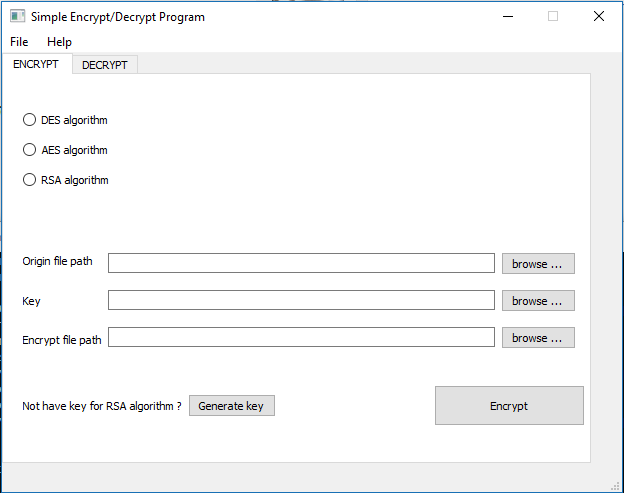
\includegraphics[scale=.5]{hinh/aes-1}
    \end{center}
    \caption{Màn hình khởi động của ứng dụng}
    \label{refhinh1}
    \end{figure}
\end{center}

%%
	\item
	Lựa chọn giải thuật AES và chọn đường dẫn file
\begin{center}
    \begin{figure}[H]
    \begin{center}
     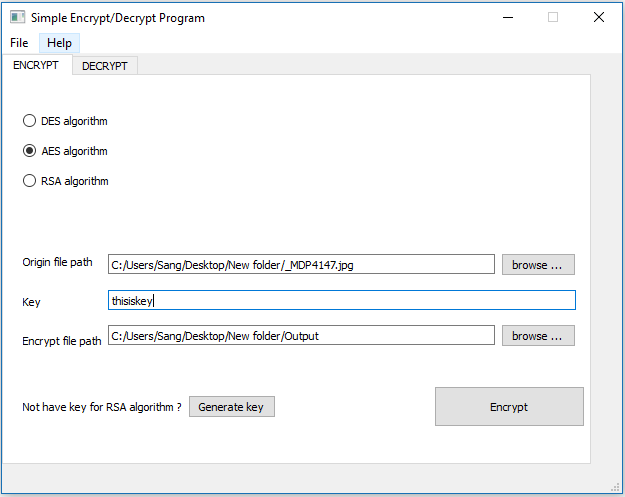
\includegraphics[scale=.5]{hinh/aes-2}
    \end{center}
    \caption{Nhập đường dẫn tệp, khóa và địa chỉ lưu tệp đã mã hóa cho giải thuật AES}
    \label{refhinh2}
    \end{figure}
\end{center}
%%
	\item
Nhấn Encrypt để mã hóa file
\begin{center}
    \begin{figure}[H]
    \begin{center}
     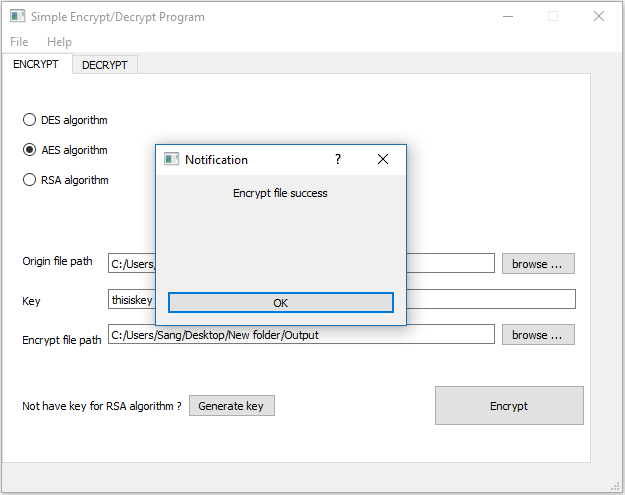
\includegraphics[scale=.5]{hinh/aes-3}
    \end{center}
    \caption{Mã hóa tệp thành công}
    \label{refhinh3}
    \end{figure}
\end{center}
	\end{itemize}

\subsection{Mã hóa bằng giải thuật DES3} 
\begin{itemize}
\item
Lựa chọn giải thuật DES và chọn đường dẫn file
\begin{center}
    \begin{figure}[H]
    \begin{center}
     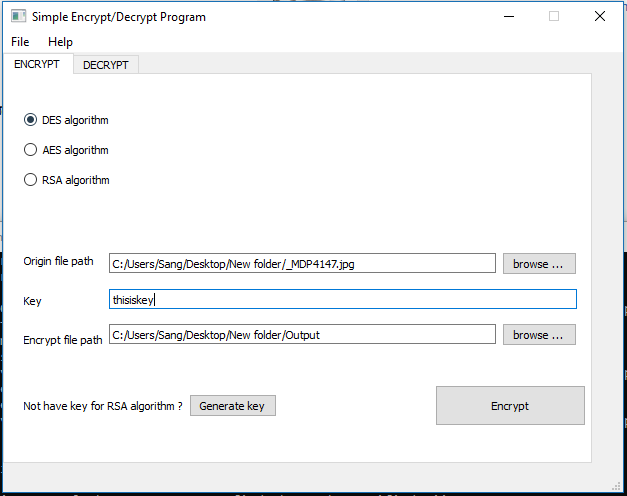
\includegraphics[scale=.5]{hinh/des-2}
    \end{center}
    \caption{Nhập đường dẫn tệp, khóa và địa chỉ lưu tệp đã mã hóa cho giải thuật DES3}
    \label{refhinh4}
    \end{figure}
\end{center}
\item
Nhấn Encrypt để mã hóa file
\begin{center}
    \begin{figure}[H]
    \begin{center}
     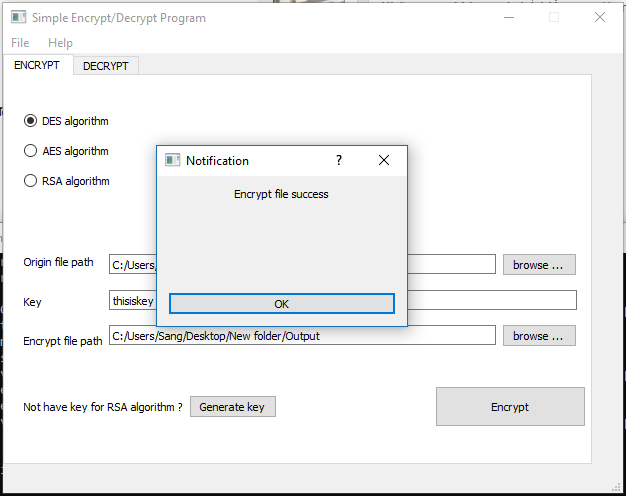
\includegraphics[scale=.5]{hinh/des-3}
    \end{center}
    \caption{Mã hóa tệp thành công}
    \label{refhinh5}
    \end{figure}
\end{center}
\end{itemize}

\subsection{Mã hóa bằng giải thuật RSA}
\begin{itemize}
	
    \item
    Chọn đường dẫn file cần mã hóa
    \begin{center}
    \begin{figure}[H]
    \begin{center}
     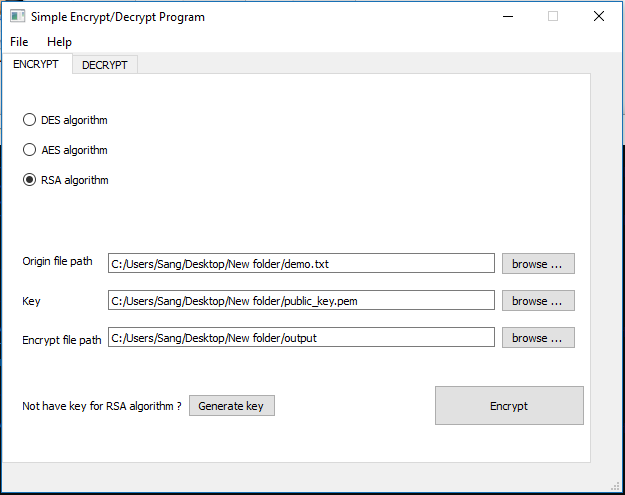
\includegraphics[scale=.5]{hinh/rsa-1}
    \end{center}
    \caption{Nhập đường dẫn tệp, đường dẫn khóa, đường dẫn của thư mục lưu tệp đã mã hóa}
    \label{refhinh6}
    \end{figure}
	\end{center}
	\item
	Chọn ENCRYPT
	\begin{center}
    \begin{figure}[H]
    \begin{center}
     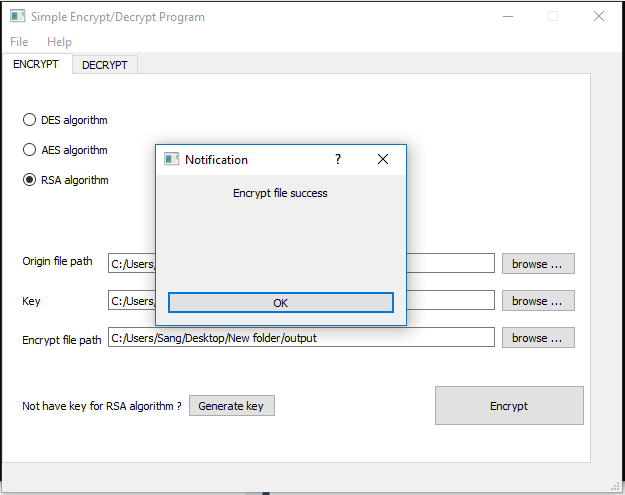
\includegraphics[scale=.5]{hinh/rsa-2}
    \end{center}
    \caption{Mã hóa tệp thành công}
    \label{refhinh7}
    \end{figure}
	\end{center}
\end{itemize}
%%%%%%%%%%%%%%%%%
%%%%%%%%%%%%%%%%%

	\subsection{Giải mã bằng giải thuật AES}
	\begin{itemize}
	
%%
	\item
	Lựa chọn giải thuật AES và chọn đường dẫn file
\begin{center}
    \begin{figure}[H]
    \begin{center}
     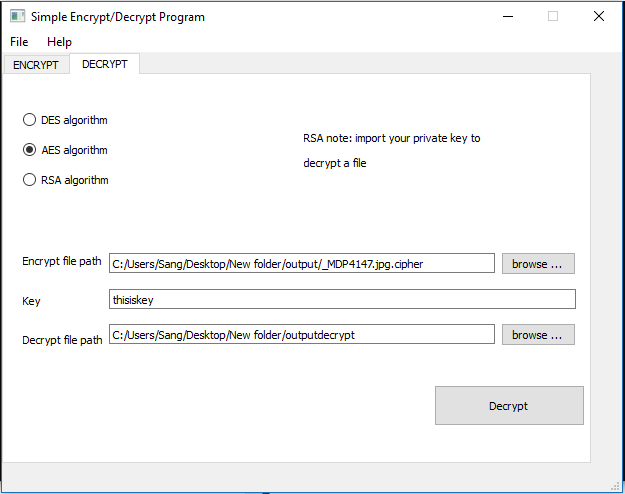
\includegraphics[scale=.5]{hinh/decrypt-aes-1}
    \end{center}
    \caption{Chọn đường dẫn của tệp cần giải mã, khóa, thư mục lưu}
    \label{refhinh8}
    \end{figure}
\end{center}
%%
	\item
Nhấn Decrypt để giải mã file
\begin{center}
    \begin{figure}[H]
    \begin{center}
     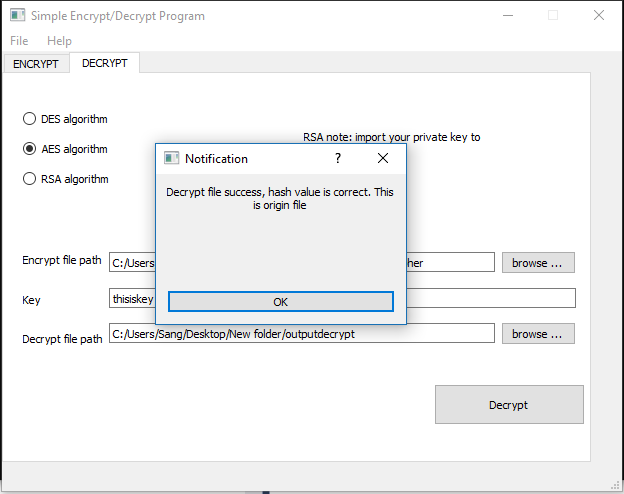
\includegraphics[scale=.5]{hinh/decrypt-aes-2}
    \end{center}
    \caption{Kết quả kiểm tra hàm hash của tệp vừa được giải mã}
    \label{refhinh9}
    \end{figure}
\end{center}
	\end{itemize}

\subsection{Giải mã bằng giải thuật DES3} 
\begin{itemize}
\item
Lựa chọn giải thuật DES và chọn đường dẫn file
\begin{center}
    \begin{figure}[H]
    \begin{center}
     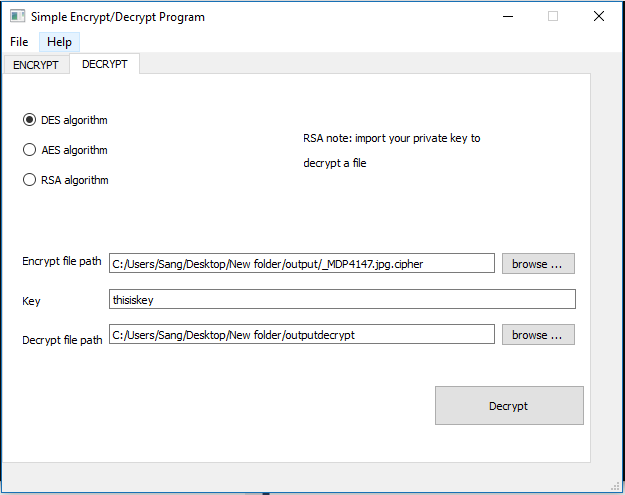
\includegraphics[scale=.5]{hinh/decrypt-des-1}
    \end{center}
    \caption{Chọn đường dẫn của tệp cần giải mã, khóa, thư mục lưu của giải thuật DES3}
    \label{refhinh10}
    \end{figure}
\end{center}
\item
Nhấn Decrypt để giải mã file
\begin{center}
    \begin{figure}[H]
    \begin{center}
     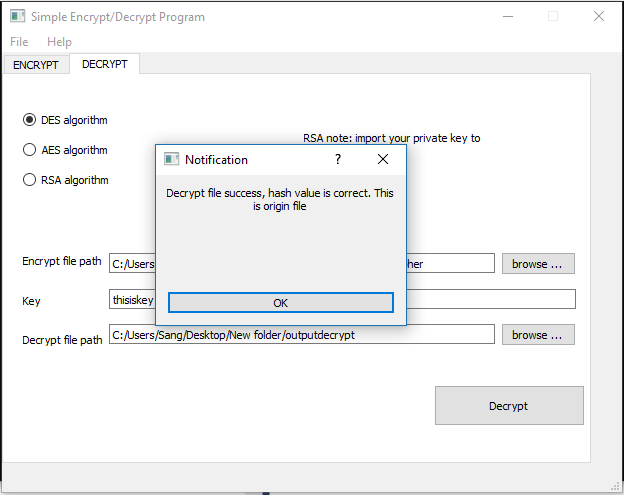
\includegraphics[scale=.5]{hinh/decrypt-des-2}
    \end{center}
    \caption{Hiển thị kết quả giải mã, kết quả của hàm hash}
    \label{refhinh11}
    \end{figure}
\end{center}
\end{itemize}

\subsection{Giải mã bằng giải thuật RSA}
\begin{itemize}
\item
	Lựa chọn giải thuật RSA và chọn đường dẫn file
\begin{center}
    \begin{figure}[H]
    \begin{center}
     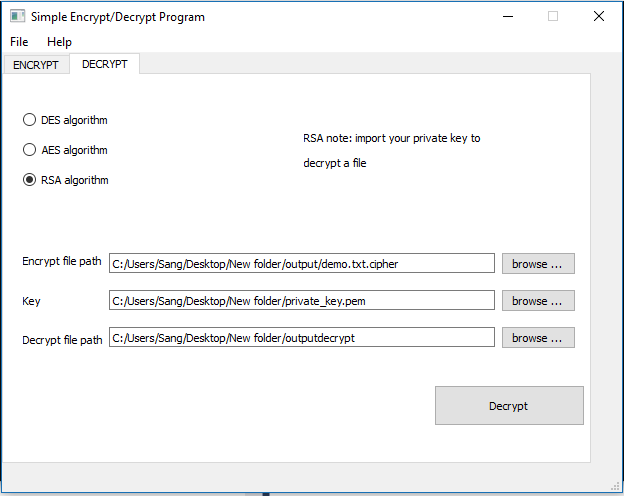
\includegraphics[scale=.5]{hinh/decrypt-rsa-1}
    \end{center}
    \caption{Chọn đường dẫn của tệp cần giải mã, đường dẫn khóa, địa chỉ lưu}
    \label{refhinh12}
    \end{figure}
\end{center}
\item
Nhấn Decrypt để giải mã file
\begin{center}
    \begin{figure}[H]
    \begin{center}
     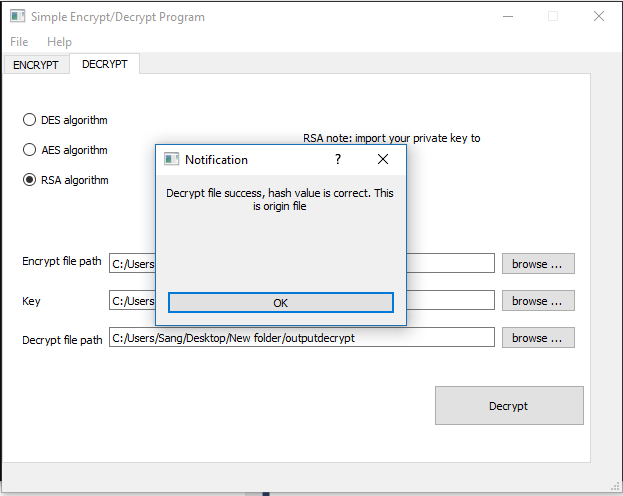
\includegraphics[scale=.5]{hinh/decrypt-rsa-2}
    \end{center}
    \caption{Kết quả giải mã và kiểm tra của hám hash}
    \label{refhinh13}
    \end{figure}
\end{center}
\end{itemize}

\section{Hướng phát triển}

	\begin{itemize}
	  	\item
			Củng cố phần giao diện
	  	\item
			Xây dựng thanh tiến trình khi đang mã hóa
	  	\item
			Xây dựng một gói cài đặt ứng dụng, để người dùng dễ dàng cài đặt
	\end{itemize}


\section{Đánh giá hoạt động các thành viên trong nhóm}
	\begin{itemize}
		\item
		Dương Tấn Sang: 33,33 \%
		\item
		Ngô Thiên Tín: 33,33 \%
		\item
		Lê Bá Anh Tuấn: 33,33 \%
	\end{itemize}	
\newpage
\newpage
%%%%%%%%%%%%%%%%%%%%%%%%%%%%%%%%%


%%%%%%%%%%%%%%%%%%%%%%%%%%%%%%%%%
\begin{thebibliography}{80}


\bibitem{PyCryptodome}
PyCryptodome
``\textbf{https://www.pycryptodome.org/en/latest}'', 


\bibitem{PyQt4}
PyQt4
``\textbf{http://pyqt.sourceforge.net/Docs/PyQt4/}'', 



\end{thebibliography}
\end{document}
